%% Copernicus Publications Manuscript Preparation Template for LaTeX Submissions
%% ---------------------------------
%% This template should be used for copernicus.cls
%% The class file and some style files are bundled in the Copernicus Latex Package, which can be downloaded from the different journal webpages.
%% For further assistance please contact Copernicus Publications at: production@copernicus.org
%% http://publications.copernicus.org/for_authors/manuscript_preparation.html


%% Please use the following documentclass and journal abbreviations for discussion papers and final revised papers.


% arara: pdflatex: { synctex: on }
% arara: bibtex
% arara: pdflatex: { synctex: on }
% arara: pdflatex: { synctex: on }

%% 2-column papers and discussion papers
\documentclass[gmd, manuscript]{copernicus}



%% Journal abbreviations (please use the same for discussion papers and final revised papers)

% Archives Animal Breeding (aab)
% Atmospheric Chemistry and Physics (acp)
% Advances in Geosciences (adgeo)
% Advances in Statistical Climatology, Meteorology and Oceanography (ascmo)
% Annales Geophysicae (angeo)
% ASTRA Proceedings (ap)
% Atmospheric Measurement Techniques (amt)
% Advances in Radio Science (ars)
% Advances in Science and Research (asr)
% Biogeosciences (bg)
% Climate of the Past (cp)
% Drinking Water Engineering and Science (dwes)
% Earth System Dynamics (esd)
% Earth Surface Dynamics (esurf)
% Earth System Science Data (essd)
% Fossil Record (fr)
% Geographica Helvetica (gh)
% Geoscientific Instrumentation, Methods and Data Systems (gi)
% Geoscientific Model Development (gmd)
% Geothermal Energy Science (gtes)
% Hydrology and Earth System Sciences (hess)
% History of Geo- and Space Sciences (hgss)
% Journal of Sensors and Sensor Systems (jsss)
% Mechanical Sciences (ms)
% Natural Hazards and Earth System Sciences (nhess)
% Nonlinear Processes in Geophysics (npg)
% Ocean Science (os)
% Proceedings of the International Association of Hydrological Sciences (piahs)
% Primate Biology (pb)
% Scientific Drilling (sd)
% SOIL (soil)
% Solid Earth (se)
% The Cryosphere (tc)
% Web Ecology (we)
% Wind Energy Science (wes)


%% \usepackage commands included in the copernicus.cls:
%\usepackage[german, english]{babel}
%\usepackage{tabularx}
%\usepackage{cancel}
%\usepackage{multirow}
%\usepackage{supertabular}
%\usepackage{algorithmic}
%\usepackage{algorithm}
%\usepackage{amsthm}
%\usepackage{float}
%\usepackage{subfig}
%\usepackage{rotating}


\begin{document}

\title{A 1-Dimensional Sympagic-Pelagic-Benthic transport model (\textrm{SPBM}) v0.2: Coupled simulation of ice, water column, and sediment biogeochemistry, suitable for Arctic applications}


% \Author[affil]{given_name}{surname}

\Author[1]{Shamil}{Yakubov}
\Author[2]{Philip}{Wallhead}
\Author[3,4]{Elizaveta}{Protsenko}
\Author[3,4]{Evgeniy}{Yakushev}
\Author[4]{Svetlana}{Pakhomova}

\affil[1]{Institute of Coastal Research, Helmholtz-Zentrum Geesthacht (HZG), Geesthacht, Germany}
\affil[2]{Norwegian Institute for Water Research (NIVA vest), Thorm{\o}hlensgate 53 D, 5006, Bergen, Norway}
\affil[3]{Norwegian Institute for Water Research (NIVA), Gaustadall{\'e}en 21, 0349, Oslo, Norway}
\affil[4]{P.P.Shirshov Institute of Oceanology RAS, Nakhimovskiy prosp. 36,
117991, Moscow, Russia}

%% The [] brackets identify the author with the corresponding affiliation. 1, 2, 3, etc. should be inserted.



\runningtitle{A 1-Dimensional Sympagic-Pelagic-Benthic transport model}

\runningauthor{Sh.Yakubov, Ph.Wallhead, E.Protsenko, E.Yakushev, S.Pakhomova}

\correspondence{Shamil Yakubov (shamil.yakubov@hzg.de)}



\received{}
\pubdiscuss{} %% only important for two-stage journals
\revised{}
\accepted{}
\published{}

%% These dates will be inserted by Copernicus Publications during the typesetting process.


\firstpage{1}

\maketitle



\begin{abstract}

Marine biogeochemical processes can strongly interact with processes occurring in adjacent ice and sediments.
This is especially likely in areas with shallow water and frequent ice cover, both of which are common in the Arctic.
Modelling tools are therefore required to simulate coupled biogeochemical systems in ice, water, and sediments domains.
We developed a 1D Sympagic-Pelagic-Benthic transport model (\textrm{SPBM}) which uses input from physical model simulations to describe hydrodynamics and ice growth and modules from the Framework for Aquatic Biogeochemical Models (\textrm{FABM}) to construct a user-defined biogeochemical model.
\textrm{SPBM} simulates the processes of vertical diffusion, sinking/burial, and biogeochemical transformations within and between the three domains.
The potential utility of \textrm{SPBM} is demonstrated herein with two test runs using modules from the European Regional Seas Ecosystem Model (\textrm{ERSEM}) and the Bottom-RedOx Model biogeochemistry (\textrm{BROM}-biogeochemistry).
The first run simulates multiple phytoplankton functional groups inhabiting the ice and water domains, while the second simulates detailed redox biogeochemistry in the ice, water, and sediments.
\textrm{SPBM} is a flexible and computationally-efficient tool for integrated simulation of ice, water, and sediment biogeochemistry, and as such may help in producing well-parameterized biogeochemical models for regions with strong sympagic-pelagic-benthic interactions.

\end{abstract}


%%\copyrightstatement{TEXT}


\introduction  %% \introduction[modified heading if necessary]

Arctic marine ecosystems have undergone drastic changes and the most important changes are climatically driven~\citep{Schofield2010,Bellerby2005,Bellerby2012,Denman2011,Silyakova2013}.
The Coupled Model Intercomparison Project and the Community Climate System Model studies have projected atmospheric warming in the Arctic of 1.5 - 4.5 times the mean global warming, and the Arctic marine environment is expected to be strongly impacted by a loss of ice cover, increasing light exposure, ocean warming, freshening, acidification, and deoxygenation~\citep{Holland2003}.
Modelling simulations are needed for the analysis of present conditions and the projection of long-term impacts on Arctic marine biogeochemistry.

A biogeochemical model suitable for the Arctic should take into account the specific conditions of this region, such as the seasonal to permanent ice cover and the presence of shelf areas.
Thus, the model should preferably combine processes occurring in 3 domains: ice, water column, and sediments.
Each of these domains has some specific features and modelling challenges:

\emph{Ice}.
The Arctic ice-algal primary production is a significant part of the total primary production of the Arctic region~\citep{Arrigo2010}.
Photosynthetic microorganisms extend the production season, provide a winter and early spring food source, and contribute to organic carbon export to depth~\citep{Vancoppenolle2013}.
A modelling study~\citep{Jin2012} estimated an average Arctic ice-algal primary production of 21.7 \unit{Tg\,C\,year^{-1}}, which equates to roughly 5\% of total pelagic primary production~\citep{Duarte2015} for this area.
\citet{Arrigo2010} estimates sea ice algal production accounting for 5~\% - 10~\% of total Arctic and Southern Ocean primary productivity.
Another modelling study suggested that under a mild climate change scenario the sea ice community around Greenland may become generally more productive while pelagic phytoplankton productivity may decrease~\citep{Tedesco2012}.
It is therefore desirable to include the ice domain in biogeochemical modelling studies of the Arctic region.
There are 3 main approaches to implement ice algae behaviour according to the place where algae live in the ice column~\citep{Tedesco2014, Vancoppenolle2017}:
in the bottom layer of an ice column with fixed thickness,
in the bottom layer of an ice column with variable thickness,
or in any layer of an ice column.
Recent research suggests that ice-algal models should resolve vertically the ice to avoid biases that may result from either assuming that ice algae are solely present at the bottom layer or that they have a homogeneous vertical distribution~\citep{Duarte2015}.

\emph{Water column}.
In the Arctic, global change is causing seawater acidification, accompanied by local changes in productivity and oxygen depletion~\citep{Bopp2013,Henson2017}.
It follows that the carbon cycle can be an important component of multidecadal-scale biogeochemical models.
Oxygen dynamics and redox process parameterization can also be useful in areas affected by oxygen depletion (often in estuaries and fjords).
To improve the representation of near-bottom processes the Benthic Boundary Layer~(\textrm{BBL}) should be incorporated into the water column domain.
The \textrm{BBL} is "the part of the marine environment that is directly influenced by the presence of the interface between the bed and its overlying water"~\citep{Dade2001}.
For the Arctic, this layer is especially important since ice melting and permafrost thawing can drive strong fluxes of ungrazed organic material to the \textrm{BBL}~\citep{Lonne1999}.

\emph{Sediments}.
Sinking fluxes from the water column can provide sources of new energy for the benthic community.
Also, it has been shown that benthic, as well as pelagic activity,  can be an important factor for annual pH variability in coastal areas~\citep{Blackford2007}.
Sediment layers in models should therefore respond accurately to sinking fluxes and provide accurate remineralization rates.
Redox processes occurring in sediments can be highly structured in the vertical, suggesting a need for explicit vertical resolution in sediment models.

In view of these features and challenges, we aimed to develop a flexible and computationally-efficient 1D vertical transport-reaction model that can provide integrated simulation of biogeochemical processes in ice, water column, and sediments domains, with a vertically-resolved grid for each.
The resulting Sympagic-Pelagic-Benthic Model (\textrm{SPBM}) uses \textrm{NetCDF} file inputs from hydrodynamic/ice models to describe an "offline" physical environment, and the Framework for Aquatic Biogeochemical Models (\textrm{FABM})~\citep{Bruggeman2014} to provide biogeochemical source-minus-sink terms and vertical sinking velocities.
The \textrm{FABM} coupling allows the user to construct their own biogeochemical model using existing modules in the \textrm{FABM} library plus any new modules written by the user (\textrm{SPBM} does not itself provide any new biogeochemical modules).
The \textrm{FABM} library is rapidly expanding and presently includes modules from some of the most detailed published biogeochemical models, e.g. The European Regional Seas Ecosystem Model (\textrm{ERSEM})~\citep{ersem2016}, the Bottom RedOx Model - biogeochemistry (\textrm{BROM}-biogeochemistry)~\citep{Yakushev2017}, the PCLake aquatic ecosystem model~\citep{Hu2016}, and the Model for Adaptive Ecosystems in Coastal Seas (\textrm{MAECS})~\citep{Wirtz2016, Kerimoglu2017}.
As with \textrm{FABM}, \textrm{SPBM} transport code is written in object-oriented Fortran language.

The paper is structured as follows:
Section 1 - Introduction (this part);
Section 2 - A detailed description of the \textrm{SPBM} routines;
Section 3 - Results from two test simulations to demonstrate \textrm{SPBM}'s capabilities and its relevance to Arctic biogeochemical modelling;
Section 4 - A discussion of \textrm{SPBM} capabilities and limitations;
Section 5 - Conclusions.

\section{\textrm{SPBM}: A 1D transport model}

\textrm{FABM} provides three types of model variables: state variables, diagnostic variables, and dependencies.
State variables are the basic elements for which the rates of changes are provided.
Diagnostic variables are calculated in the biogeochemical models according to the values of the state variables at each time step.
Dependencies are the physical environment variables and interconnections within \textrm{FABM}.
\textrm{SPBM} operates with state variables, sends dependencies to \textrm{FABM}, and outputs all necessary state and diagnostic variables in \textrm{NetCDF} files.
Within \textrm{SPBM}, state variables are considered as solute or particulate concentrations.

\subsection{Formulation and numerical integration}
\label{subsec:Formulation}

\textrm{SPBM} solves a system of 1-D transport equations in Cartesian coordinates for all three domains (ice, water column, and sediments).
The dynamics are
\begin{equation}
    \frac{\partial{C_{i}}}{\partial{t}}
    = \frac{\partial{}}{\partial{z}} A_{f} D
    \frac{\partial{C_{i}P_{f}}}{\partial{z}}
    -\frac{\partial{}}{\partial{z}} u C_{i}
    +R_{i}
    \label{eq:1}
\end{equation}
where
$C_{i}$ is the concentration of the \textit{i\/}th state variable in units provided by the biogeochemical model through \textrm{FABM}, \newline [\unit{mmol\,m^{-3}\,total\,volume}] or [\unit{mg\,m^{-3}\,total\,volume}];
$t$ is the time step, [\unit{s}];
$z$ is the depth, [\unit{m}];
$A_{f}$ is the porosity-related area restriction factor for fluxes, dimensionless;
$D$ is the total diffusivity, [\unit{m^{2}\,s^{-1}}];
$P_{f}$ is the porosity factor, dimensionless;
$u$ is the sinking velocity (advection / burial in the sediments), [\unit{m\,s^{-1}}].
$R_{i}$ is the combined sources minus sinks of the \textit{i\/}th state variable provided by the biogeochemical model through \textrm{FABM}, [\unit{mmol\,m^{-3}\,total\,volume\,s^{-1}}] or [\unit{mg\,m^{-3}\,total\,volume\,s^{-1}}];

The porosity factor $P_{f}$ is used to calculate the volume concentration in brine (in the ice column) or in pore water / solid matrix in the sediments.
Exchange within the ice and sediment layers occurs through brine channels and through pores or solid matrix, so the area restriction factor $A_{f}$ is included to limit fluxes within the respective phases (intraphase mixing).
The values of $A_{f}$, $P_{f}$, $D$ and $u$ depend on whether these parameters are calculated in ice, water column, or sediment domains and whether the state variable is solute or particulate.

\emph{In the ice domain:}

For particulates, it is assumed that the concentration is the same in both the brine channels and ice matrix, hence $P_{f} = 1$.
However, vertical fluxes are assumed to be restricted to the brine channels where the particulates are mobilised in suspension, hence $A_{f} = \varphi(z)$.
Here, the dimensionless porosity $\varphi(z)$ is equal to the relative volume of the brine channels in the ice~\citep{Arrigo1993}, which can be obtained from an ice thermodynamic model or using empirical relationships (see Appendix~\ref{app:A}).
Solutes are assumed to be excluded from the ice matrix, hence $P_{f} = \frac{1}{\varphi(z)}$, and fluxes are again restricted to the brine channels, hence $A_{f} = \varphi(z)$.
The total diffusivity $D$ in the ice brine channels is a sum of the molecular diffusivity $D_{m}(s)$ [\unit{m^{2}\,s^{-1}}] on the ice-water interface, the gravity drainage diffusivity $D_{gd}(z)$ [\unit{m^{2}\,s^{-1}}] at depths $z$ within the ice, and the diffusivity caused by convection that occurs in the bottom layer of the growing ice $D_{gi}(s)$ [\unit{m^{2}\,s^{-1}}]~\citep{Arrigo1993}:
\begin{align}
    &D = D_{m}(s) + D_{gd}(z) + D_{gi}(s)\\
    &D_{gd}(z) = F_{vb} z_{b}\\
    &D_{gi}(s) = 10^{-2} z_{s} (9.667 \cdot 10^{-9}
    + 4.49 \cdot 10^{-6}IceGrowth
    - 1.39 \cdot 10^{-7}IceGrowth^{2})
\end{align}

where $s$ means that the value of the parameter is determined only on the interface between the bottom (\textit{s}\/keletal) layer of ice and surface water layer;
$F_{vb}$ is a constant mean flux volume rate from the brine channels, [\unit{m\,s^{-1}}];
$z_{b}$ is the vertical distance over which the ice column is influenced by brine tube convection (depths where $\varphi(z) > \varphi_{min}$), [\unit{m}];
$IceGrowth$ is the total ice growth rate [\unit{cm\,sec^{-1}}];
$z_{s}$ is the thickness of the ice layer, [\unit{m}].
$D_{gi}(s)$ is not equal to zero only during the period of ice build-up and only on the interface between water and ice.
Alternatively, the total diffusivity $D$ can be read from an input file generated by e.g. an ice thermodynamic model.

The sinking velocity $u$ is non-zero only for particulate variables in the layers where $\varphi(z) > \varphi_{min}$ (if $\varphi(z) \leqslant \varphi_{min}$ sea ice brine pockets are not interconnected) and is generally determined at each time step by the biogeochemical model through \textrm{FABM}.
For all diatoms living in the ice column, to represent their ability to maintain their vertical position relative to the skeletal layer~\citep{Arrigo1993}, $u$ is set to a constant but possibly layer-dependent value within the ice column and zero on the ice-water interface between ice and water domains, while the total diffusivity $D$ is set to zero.

\emph{In the water column domain:}

Here $P_{f} = 1$ and $A_{f} = 1$ at all depths for both solutes and particulates, since there is only one phase to consider.

The total diffusivity $D$ is composed of the molecular diffusivity $D_{0}$ [\unit{m^{2}\,s^{-1}}] and the turbulence diffusivity $D_{t}(z)$ [\unit{m^{2}\,s^{-1}}]:
\begin{equation}
    D = D_{0} + D_{t}(z)
\end{equation}

$D_{t}(z)$ is taken from the hydrophysical model as input data.
The water column domain contains the structure that could be called the \textrm{BBL}.
It is located in the lower part of the water column (see Subsect.~\ref{subsec:Grid}).
Turbulent diffusivity for each layer $z_{i}$ within the BBL is linearly decreasing from the deepest non-zero value of the diffusivity $D_{t}(z_{d})$ as follows:
\begin{equation}
    D_{t}(z_{i}) = \frac{D_{t}(z_{d})}
    {z_{d} - z_{0}}
    (z_{i} - z_{0})
\end{equation}

where $z_{d}$ [\unit{m}] is the deepest depth with non-zero value of $D_{t}(z)$ and $z_{0}$ [\unit{m}] is the bottom depth.

The sinking velocity $u$ is taken from the biogeochemical model through \textrm{FABM} for all particulates, and is zeros for all solutes.

\emph{In the sediments domain:}

Within the sediments, particulate variables are confined to the sediment matrix and solutes are confined to the pore water.
So for solid particulates the porosity factor $P_{f} = \frac{1}{1 - \varphi(z)}$ and the area restriction factor $A_{f} = 1 - \varphi(z)$ at depths $z$.
For solutes $P_{f} = \frac{1}{\varphi(z)}$ and $A_{f} = \varphi(z)$.
There is no adsorption in the present version.

A time-independent porosity $\varphi(z)$ at depths $z$ through the entire sediments domain is described following~\citet{Soetaert1996}:
\begin{equation}
    \varphi(z) = \varphi(z_{\infty})
    + (\varphi(z_{0}) - \varphi(z_{\infty}))
    \mathrm{e}^{-\frac{(z - z_{swi})}{k_{\varphi}}}
\end{equation}

where $\varphi(z_{\infty})$ is the deep porosity, dimensionless;
$\varphi(z_{0})$ is the porosity at the sediment-water interface (\textrm{SWI}), dimensionless;
$z_{swi}$ is the depth of the \textrm{SWI}, [\unit{m}];
$k_{\varphi}$ is the coefficient for exponential porosity change, [\unit{m}].

The total diffusivity $D$ is a sum of the molecular diffusivity $D_{m}(z)$ [\unit{m^{2}\,s^{-1}}] and the bioturbation diffusivity $D_{b}(z)$ [\unit{m^{2}\,s^{-1}}]~\citep{Boudreau1997}:
\begin{align}
                            &D = D_{m}(z) + D_{b}(z) \\
    \text{for solutes: }    &D_{m}(z) = D_{0} \frac{1}{1 - 2 \ln \varphi(z)} \mu_{d} \\
    \text{for particulates: }     &D_{m}(z) = 0 \\
                            &D_{b}(z) = D_{bo}(z)
    \frac{\chem{O_{2}}}{\chem{O_{2}} + K_{\chem{O_{2}}}}
\end{align}

where $D_{0}$ is the infinite-dilution molecular diffusivity, [\unit{m^{2}\,s^{-1}}];
$\mu_{d}$ is the relative dynamic viscosity, dimensionless;
$\chem{O_{2}}$ is the oxygen concentration in the bottom layer of the water column, [\unit{mmol\,m^{-3}}];
$K_{\chem{O_{2}}}$ is the half-saturation constant, [\unit{mmol\,m^{-3}}].
The oxygen-saturated bioturbation diffusivity~\citep{Yakushev2017} $D_{bo}(z)$ [\unit{m^{2}\,s^{-1}}] depends on the distance $z_{db}(z)$ [\unit{m}] between the interface depth $z$ and the depth with a constant bioturbation activity as follows:
\begin{align}
    &z_{db}(z) = z - (z_{swi} + z_{cb}) \\
    \text{if $z < z_{swi} + z_{cb}$: } &D_{bo}(z) = D_{bm} \\
    \text{if $z > z_{swi} + z_{cb}$: } &D_{bo}(z) = D_{bm}
    \mathrm{e}^{- \frac{z_{db}(z)}{F_{d}}}
\end{align}

where $z_{swi}$ is the depth at the \textrm{SWI}, [\unit{m}];
$z_{cb}$ is the constant bioturbation activity layer thickness, [\unit{m}];
$D_{bm}$ is the maximum bioturbation diffusivity, [\unit{m^{2}\,s^{-1}}];
$F_{d}$ is the bioturbation decay scale, [\unit{m}].

On the \textrm{SWI} it is assumed that the bioturbation diffusivity mixes concentrations in units [\unit{mmol\,m^{-3}\,total\,volume}] instead of [\unit{mmol\,m^{-3}\,solids/solutes}] (interphase mixing).
Therefore special values of $P_{f}$ are needed for the layers immediately above and below the \textrm{SWI} (see Appendix~\ref{app:B}):
\begin{align}
    \text{for solutes: } &P_{f}(z_{a,b}) =
    \frac{\frac{\varphi_{swi}}{\varphi_{a,b}} D_{m}(z_{swi}) + D_{b}(z_{swi})}
    {\varphi_{swi} ( D_{m}(z_{swi}) + D_{b}(z_{swi}) )} \\
    \text{for solids: } &P_{f}(z_{a,b}) = \frac{1}{1 - \varphi_{swi}}
\end{align}

where the subscripts $a$, $b$ and $swi$ determine a location of the corresponding variables: $a$ means the layer above, $b$ - the layer below, $swi$ - on the \textrm{SWI}.

The advection/burial velocities $u(z)$ are described following~\citet{Yakushev2017}:
\begin{align}
\begin{split}
\label{eq:advection}
    & \text{for solutes: } u(z) =
    \frac{\varphi(z_{\infty})}{\varphi(z)} u_{b} +
    \frac{1}{\varphi(z)} D_{b}^{inter}
    \frac{\partial \varphi(z)}{\partial z}
\end{split} \\
     & \text{for particulates: } u(z) =
    \frac{1 - \varphi(z_{\infty})}{1 - \varphi(z)} u_{b} -
    \frac{1}{1 - \varphi(z)} D_{b}^{inter}
    \frac{\partial \varphi(z)}{\partial z}
\label{eq:burial}
\end{align}

where $u_{b}$ is the deep burial velocity, [\unit{m\,s^{-1}}];
$D_{b}^{inter}$ is the interphase component of the total bioturbation diffusivity $D_{b} = D_{b}^{intra} + D_{b}^{inter}$, and $D_{b}^{inter}$ is nonzero only on the \textrm{SWI} where $D_{b}^{inter} = D_{b}$ [\unit{m^{2}\,s^{-1}}].
Note that although a non-zero $D_{b}^{inter}$ beyond the \textrm{SWI} would alter the computed advection/burial velocities $u(z)$ via Eqns. (\ref{eq:advection}, \ref{eq:burial}), the net transport of biogeochemical tracers would not be affected because corresponding interphase components $\frac{1}{\varphi} C_{i} D_{b}^{inter} \frac{\partial \varphi}{\partial z}$ and $\frac{1}{1 - \varphi} C_{i} D_{b}^{inter} \frac{\partial(1 - \varphi)}{\partial z}$ would need to be added to the diffusive fluxes in Eq.~\ref{eq:1}, and these will exactly cancel the contributions of $D_{b}^{inter}$ to advection/burial.
In other words, when the porosity profile is specified and used to compute advection/burial velocities under steady state compaction, the tracer advection/diffusion depends only on the total bioturbation diffusivity, and the intraphase form assumed by \textrm{SPBM} for diffusion inside the sediments is correct irrespective of the relative contribution of inter- vs. intraphase mixing, see~\citep{Meysman2005}.
However, there can be no intraphase component of a Fickian particulate diffusion across the \textrm{SWI} because by definition there is no solid matrix above the \textrm{SWI} \citep{Yakushev2017}.

Equation~(\ref{eq:1}) is integrated numerically over a single combined (ice, water column, sediments) grid (see Subsect.~\ref{subsec:Grid}), using a constant model time step.
Time stepping follows an operator splitting approach~\citep{Butenschon2012}: concentrations are successively updated by contributions over one time step of diffusion, reaction, and sinking/advection/burial, in that order.
Diffusive updates are calculated by a semi-implicit central-space algorithm adapted from a routine in \textrm{BROM}-transport~\citep{Yakushev2017} which in turn was adapted from the General Ocean Turbulence Model (\textrm{GOTM})~\citep{Umlauf2005}.
Sinking/advection/burial updates are calculated using a first-order upwind differencing scheme.
Reaction updates are calculated from forward Euler time steps.

\subsection{The grid}
\label{subsec:Grid}

\textrm{SPBM} uses a fixed grid structure for the water column and sediments, and a time-dependent grid for the ice column.
The number of grid points inside the ice column can vary with time but the spacing is fixed (see Fig.~\ref{fig:grid}).
Water column layer depths [\unit{m}] are taken as input from a hydrophysical model (distances between layers can be unequal) and extra layers are incorporated in the lower part in order to fully resolve the \textrm{BBL}.
Total ice thickness [\unit{m}] for every day of simulation is also taken as input from a hydrophysical model, and the ice column is constructed using a fixed layer thickness [\unit{m}] as an input parameter.
Therefore the ice column is discretized into layers of strictly constant thickness $z_{s}$, and when the ice column grows or melts its total thickness can change only by multiples of $z_{s}$.
This simplification facilitates recalculation of the variable concentrations during melting and freezing (see Subsect.~\ref{subsec:Ice}).

\begin{figure}[htbp]
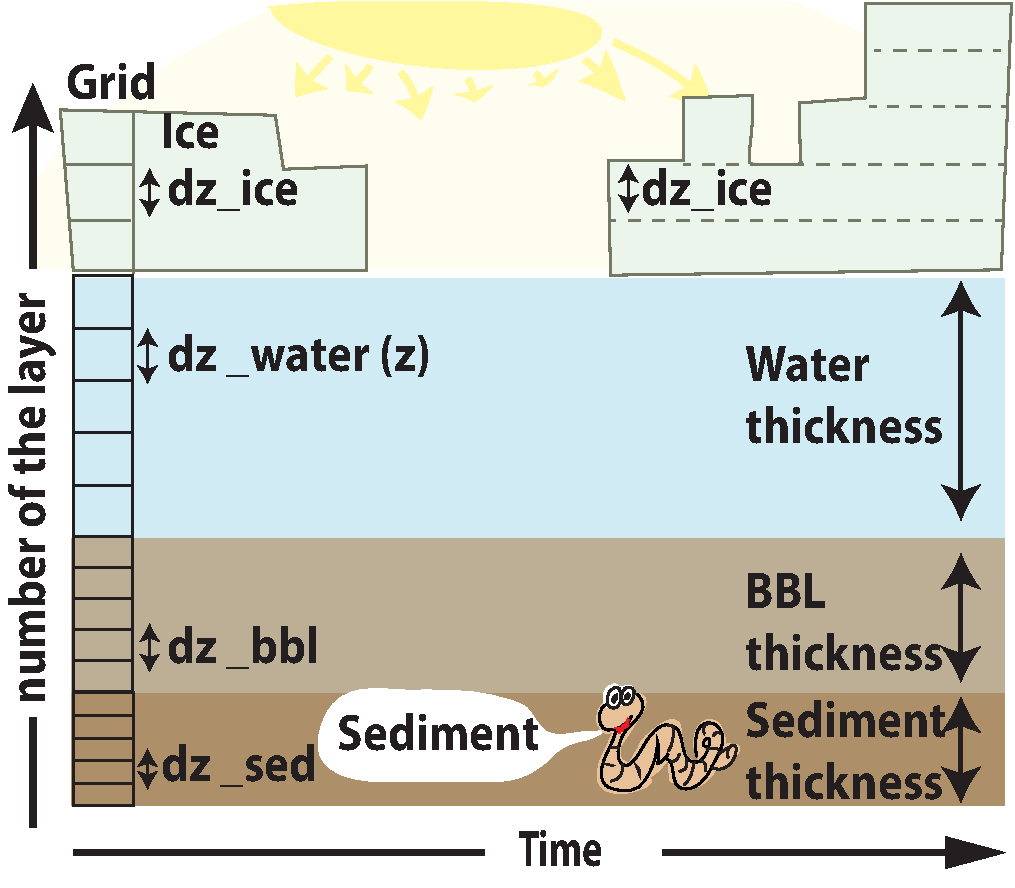
\includegraphics[width=6.3cm]{fig01}
\caption{The \textrm{SPBM} grid structure}
\label{fig:grid}
\end{figure}

\subsection{Ice column structure}
\label{subsec:Ice}
For better representation of ice algal behaviour a multilayer structure is used.
\textrm{SPBM} recalculates all state variables concentrations during freezing and melting following algorithms \ref{a1} and \ref{a2}, where $IG$ is the number of freezing (positive value) or melting (negative value) layers;
$C$ is the state variable concentration;
subscript $i$ is the layer index;
subscript $s$ is the surface water layer index;
subscript $b$ is the bottom ice layer index.
The layers are enumerated from the bottom upwards.

\begin{algorithm}[htbp]
\caption{State variable concentration recalculation during ice freezing}
\label{a1}
\begin{algorithmic}
\REQUIRE $\lvert IG \rvert > 0$
    \FOR{all $i$ in the ice domain}
        \STATE $C_{i} = C_{i - \lvert IG \rvert}$
    \ENDFOR
    \FOR{all $i$ of the new ice layers}
        \STATE $C_{i} = C_{s}$
        \STATE $C_{s} = C_{s} - C_{s}
               \frac{IceLayerWidth}{SurfaceLayerWidth}$
    \ENDFOR
\end{algorithmic}
\end{algorithm}

\begin{algorithm}[htbp]
\caption{State variable concentration recalculation during ice melting}
\label{a2}
\begin{algorithmic}
\REQUIRE $\lvert IG \rvert > 0$
    \IF{there is a diatom state variable and not the last layer has melted}
        \FOR{all $i$ of the melted ice layers}
            \STATE $C_{b} = C_{b} + C_{i}$
        \ENDFOR
        \FOR{all $i$ in the ice domain except the bottom ice layer}
            \STATE $C_{i} = C_{i + \lvert IG \rvert}$
        \ENDFOR
    \ELSE
    \FOR{all $i$ of the melted ice layers}
        \STATE $C_{s} = C_{s} + C_{i}
               \frac{IceLayerWidth}{SurfaceLayerWidth}$
    \ENDFOR
    \FOR{all $i$ in the ice domain}
        \STATE $C_{i} = C_{i + \lvert IG \rvert}$
    \ENDFOR
    \ENDIF
\end{algorithmic}
\end{algorithm}

\subsection{Irradiance formulation}
\label{subsec:Irradiance}
\textrm{FABM} biogeochemical models generally need to know the photosynthetically active radiation (\textrm{PAR}) [\unit{mol\,photons\,m^{-2}\,day^{-1}}] in each layer of the model grid.
Some \textrm{FABM} models compute water column \textrm{PAR} given only surface \textrm{PAR}, but they do not assume the existence of the ice column and consider all grid points to be located within the water column.
\textrm{SPBM} therefore provides the following simple approach to calculate \textrm{PAR} in both ice and water column domains.

\textrm{PAR} on the surface of water or ice $P_{s}$ can be calculated from the surface shortwave radiative flux~$F_{surf}$ [\unit{W\,m^{-2}}], depending on the solar declination~$k_{decl}$ [\unit{degrees}]:
\begin{align}
    &k_{decl} = 23.5 \cdot \sin{
        \frac{2 \pi JulianDay - 81}{365}} \\
    &F_{surf} = I_{m} \cos{
        \frac{\pi (latitude - k_{decl})}{180}} \\
    &P_{s} = k_{f} F_{surf}
\end{align}

where $I_{m}$ is the theoretical maximum of 24-hour average surface downwelling shortwave irradiance in air, [\unit{W\,m^{-2}}];
$k_{f}$ is the factor to convert downwelling shortwave irradiance in air to scalar \textrm{PAR} in water, [\unit{mol\,photons\,day^{-1}\,W^{-1}}]~\citep{Mobley2012}.
Alternatively, $P_{s}$ (or $F_{surf}$) can be read from an input file.

In the presence of ice, \textrm{PAR} after considering albedo influence $P_{a}$ becomes~\citep{Light2008}:
\begin{align}
    \text{if snow depth $\le$ 5 \unit{mm}: } &P_{a} =
    P_{s} k_{scatter} (1 - A_{ice}) \\
    \text{if snow depth $>$   5 \unit{mm}: } &P_{a} =
    P_{s} k_{scatter} (1 - A_{snow}) \mathrm{e}^{-k_{snow} z_{snow}}
\end{align}

where $k_{scatter}$ is the fraction of radiation transmitted through the highly scattering surface of the ice, dimensionless;
$A_{ice}$ is the ice albedo for visible light, dimensionless;
$A_{snow}$ is the snow albedo for visible light, dimensionless;
$k_{snow}$ is the snow light extinction coefficient, [\unit{m^{-1}}];
$z_{snow}$ is the snow depth, [\unit{m}].

\textrm{PAR} at any depth in the ice $P(z_{ice})$ is given by:
\begin{equation}
    P(z_{ice}) = P_{a} \mathrm{e}^{-k_{ice} z_{ice}}
\end{equation}

where $k_{ice}$ is the ice light extinction coefficient, [\unit{m^{-1}}];
$z_{ice}$ is the ice depth, [\unit{m}].

\textrm{PAR} in the water column $P(z_{water})$ is calculated according to the Beer-Lambert formulation:
\begin{align}
    \text{if there is an ice: } &P(z_{water}) =
    P(z_{IceBottom}) \mathrm{e}^{\int_{0}^{z} K_{water}(z_{water}) dz_{water}} \\
    \text{if there is no ice: } &P(z_{water}) =
    P_{s} \mathrm{e}^{\int_{0}^{z} K_{water}(z_{water}) dz_{water}}
\end{align}

where $P(z_{IceBottom})$ is the \textrm{PAR} at the ice bottom layer;
$K_{water}$ is the vertically varying water light extinction coefficient provided by the \textrm{FABM} models, describing attenuation due to living and non-living optically-active substances, [\unit{m^{-1}}];
$z_{water}$ is the water layer depth, [\unit{m}].

In the sediments domain, \textrm{PAR} equals zero in all layers.

\subsection{Initial and boundary conditions}
Initial conditions for all state variable concentrations are provided through \textrm{FABM} using its \textrm{YAML} type configuration file~\citep{Bruggeman2014}.
By default, zero gradient boundary conditions are used at upper and lower boundaries for all state variables except \chem{O_{2}} and \chem{CO_{2}}.
Diffusive fluxes of \chem{O_{2}} and \chem{CO_{2}} are provided by the biogeochemical model through \textrm{FABM} at the surface boundary (only for ice-free periods), and are set to zero at the lower boundary.
It is possible to change both boundary conditions according to the user's needs.

\subsection{The forcing data}
\label{subsec:Hydrodynamic}
\textrm{SPBM} requires time-dependent input forcings for the entire period of simulation for the water column (turbulent diffusivity [\unit{m^{2}\,s^{-1}}] on layer interfaces; temperature [\unit{C\degree}] and salinity [\unit{psu}] on layer centres) and for the ice column (total thickness [\unit{m}], snow thickness [\unit{m}], and surface temperature [\unit{C\degree}]).
Additional forcings may be required depending on the \textrm{FABM} biogeochemical models.
Downwelling shortwave radiation and \textrm{PAR} can be read from an input file instead of using the formulae provided in Subsect.~\ref{subsec:Irradiance}.
Other optional input forcings include: brine volumes and diffusion coefficients in the ice, input fluxes at the water surface, and horizontal mixing fluxes at any depth.
Input fluxes are based on concentrations $C$ which can be provided in 3 ways:
read from text or \textrm{NetCDF} file;
set as fixed sinusoidal variation in time defined by a maximum value $M$ and $Phase$ parameters ($C = 2^{-1} M + 4^{-1} M (1 + \sin{(365^{-1} \cdot 2 \pi (JulianDay - Phase)}))$);
set as fixed constant value.
$M$ and the boundary concentrations $C$ should be in units corresponding to the state variables of the appropriate \textrm{FABM} model, $Phase$ is in [\unit{days}].
\textrm{SPBM} uses input data files in \textrm{NetCDF} and text formats.

\section{Test cases}

Our test cases use forcing data from a \textrm{ROMS} simulation to provide a hydrodynamic scenario for the Laptev Sea.
A time-dependent total ice thickness and a time-independent water column structure were derived from this simulation, while the \textrm{BBL} was inserted with the following parameters: width = 50 \unit{cm}, resolution = 10 \unit{cm}. The grid in the sediments domain was continued for another 10 \unit{cm} with resolution 2 \unit{cm}.

We stress that our purpose is only to demonstrate the flexibility of \textrm{SPBM} and its relevance to Arctic marine modelling.
Rigorous, site-specific adaptation and skill assessment of particular \textrm{SPBM} configurations is not within our present remit, but is anticipated in future work.
For the test simulations, we use \textrm{FABM} to combine components from two published biogeochemical models.
Here we will explain only the most basic aspects of these models; the reader can find detailed descriptions in the provided references.
We remind that \textrm{SPBM} calculates only the transport terms in Eq.~\ref{eq:1}, while the \textrm{FABM} biogeochemical modules provide the combined sources-minus-sinks terms $R_{i}$ and the sinking velocities $u$ in the water column.
\textrm{FABM} model formulations and parameter values were derived from existing parameterizations with some limited adaptation to the Arctic scenario.

The first biogeochemical model is the European Regional Seas Ecosystem Model, \textrm{ERSEM}~\citep{ersem2016}.
Originally a coastal ecosystem model for the North Sea, \textrm{ERSEM} has evolved into a generic tool for ecosystem simulations from shelf seas to the global ocean.
Model dynamics within each functional group describe processes occurring inside a 'standard organism' \citep{Baretta1995, Vichi2007_1}.
\textrm{ERSEM} accounts for flexible elemental stoichiometry in planktonic processes by allowing decoupled fluxes of carbon, nitrogen, phosphorus, silicate, and chlorophyll a.
This requires multiple state variables to describe each functional group biomass (e.g. diatom carbon, diatom nitrogen, etc.) and results in a relatively complex model.

The second biogeochemical model is the Bottom RedOx Model (\textrm{BROM}) biogeochemistry module~\citep{Yakushev2017}.
This model represents key biogeochemical processes in the water and upper sediments, with a focus on oxygen dynamics and redox biogeochemistry.
Compared to \textrm{ERSEM}, it simulates the coupled cycles of more elements (\chem{N}, \chem{P}, \chem{Si}, \chem{C}, \chem{O}, \chem{S}, \chem{Mn}, and \chem{Fe}), resolves more structure in the bacterial community (4 functional groups vs. 1 in \textrm{ERSEM}), and calculates carbonate chemistry in more detail;
however it assumes fixed stoichiometry for all forms of organic matter (nitrogen currency), resolves only one functional group each for phytoplankton and zooplankton, and does not resolve dissolved organic matter into different lability classes.

\begin{figure}[htbp]
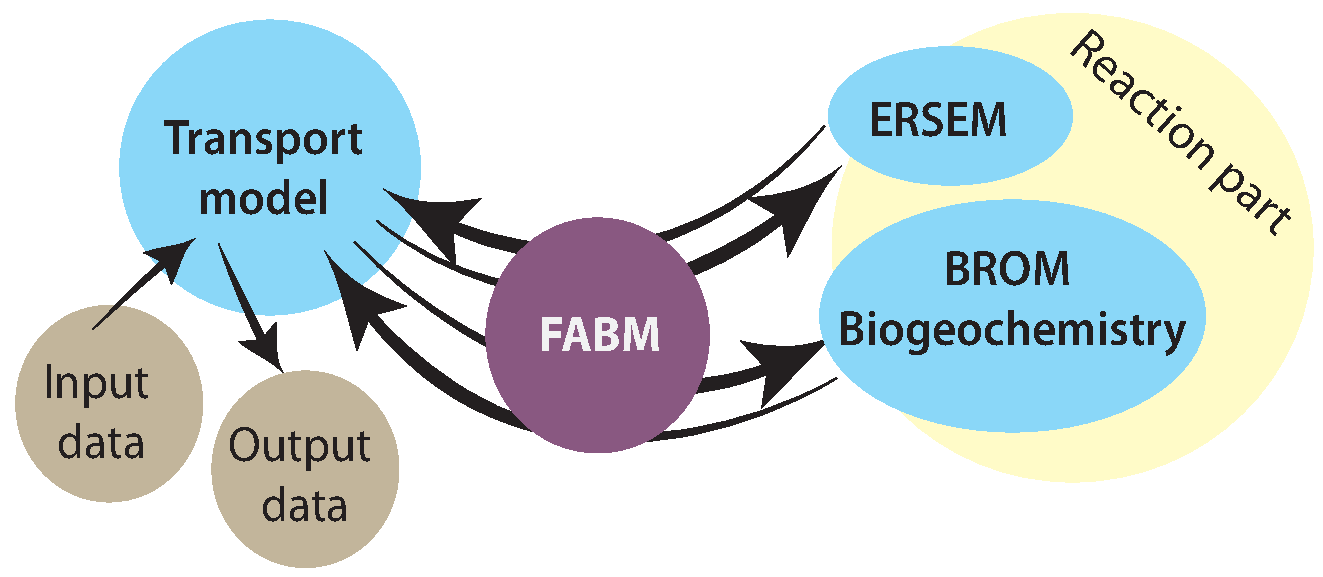
\includegraphics[width=8.3cm]{fig02}
\caption{The general scheme of models coupling}
\label{fig:General_scheme}
\end{figure}

The general coupling scheme is illustrated in Fig.~\ref{fig:General_scheme}.
A quasi-stationary solution is derived from two spin-ups, repeating the first day 100 times and then repeating the first year 10 times.
Along with \textrm{SPBM} requirements there are additional forcings required by \textrm{ERSEM} and \textrm{BROM}: wind speed [\unit{m\,s^{-1}}] and concentration of \chem{CO_{2}} in air [\unit{ppm}].
Surface shortwave radiation at sea-surface level is provided by \textrm{ROMS} and is read from an input file.

We present 2 test cases with the same hydrophysical forcings but different \textrm{FABM} model configurations.
The first demonstrates the simulation of multiple primary producer functional groups and shows their variability in contrasting conditions.
The second test case demonstrates changing redox conditions in the three domains in response to a constant input of organic matter (\textrm{OM}).
The main joint parameter values and forcing properties are provided in Appendix~\ref{app:C} (common parameters in Table~\ref{table:Common_parameters}, ice parameters in Table~\ref{table:Ice_parameters}, sediments parameters in Table~\ref{table:Sediments_parameters}, irradiance parameters are provided in Table~\ref{table:Irradiance_parameters}, and forcing properties in Table~\ref{table:properties}).

\subsection{Test case 1}
\label{subsec:tc1}

According to the~\citet{Leeuwe2018}, there are few tools yet developed to simulate different groups of ice algae.
Therefore we constructed a test case to simulate different primary producers in different ice conditions.
We used \textrm{ERSEM} primary producer functional groups with parametrizations from~\citet{ersem2016} to simulate diatoms, nanophytoplankton, picophytoplankton, and microphytoplankton.
One more algal group called ice diatoms was added, based on an original diatom primary producer parametrization which we adapted to improve growth in low irradiance conditions (see Appendix~\ref{app:D}).
Thus in total we used 5 primary producer functional groups.
All functional groups were given the same initial conditions (prior to spin-up) in both ice, water, and sediment domains;
hence differences in the steady state abundances were determined by the environment and the growth parameters/sinking velocities of the different functional groups.
All configuration files are available at the link provided in the code availability section.

\begin{figure}[htbp]
\includegraphics[width=13cm]{fig03}
    \caption{Variability of total Chl a, pH (total scale), oxygen, silicon, phosphate, nitrate}
\label{fig:ice_diatoms_nutrients}
\end{figure}

\begin{table}[H]
\centering
\caption{Comparing \textrm{SPBM} output during ice melting period with concentrations of biogeochemical tracers in sea ice and surface seawater observed for typical spring conditions in the Arctic according to~\citet[Figure 3, p.~210]{Vancoppenolle2013}}
\label{table:comparing}
\begin{tabular}{llllll}
\tophline
    Parameter: & \chem{Si} \unit{\mu M} & \chem{PO_{4}} \unit{\mu M} & \chem{NO_{3}} \unit{\mu M} & Chl a \unit{mg\,m^{-3}} & \chem{O_{2}} \unit{\mu M} \\
\middlehline
Observed in ice & - & 0 - 0.7 & 0 - 1 & 1 - 100 & 50 - 250 \\
Modelled in ice & 0.4 - 1.6 & 0.01 - 0.07 & 0 - 0.5 & 1 - 120 & 50 - 80 \\
Observed in water & - & 1.2 & 7 &  1 & 380 \\
Modelled in water & 8.5 - 9.5 & 0.34 - 0.38 & 2.5 - 2.9 & 0.1 - 0.7 & 300 - 320 \\
\bottomhline
\end{tabular}
\belowtable{} % Table Footnotes
\end{table}

Figure~\ref{fig:ice_diatoms_nutrients} shows \textrm{SPBM} output (for chlorophyll a, pH, oxygen, and nutrients) in the ice and upper water column layers during the period with maximum ice algae chlorophyll a concentrations.
This maximum is a result of thin ice (<50 \unit{cm}) during at least one month and favourable irradiance conditions.
Chlorophyll a, oxygen, and nutrients are all state variables and therefore output as concentrations per unit total volume;
pH is a diagnostic variable and is output as the negative logarithm of hydrogen ion concentrations per unit volume of brine or seawater.
The modelled values were compared with observed concentrations of biogeochemical tracers in sea ice during spring in the Arctic provided by~\citet[Figure 3, p.~210]{Vancoppenolle2013}.
Most model ranges fall inside or at least overlap the observational ranges (see Table~\ref{table:comparing}).
Also, Fig.~\ref{fig:ice_diatoms_nutrients} shows that the modelled vertical distributions in sea ice reproduce some commonly observed features~\citep{Vancoppenolle2013}:
during ice melt chlorophyll a concentrations are highest in the bottom layer;
during freezing the pH increases in the upper ice layers, reaching values higher then 10 during winter (see supplementary material) in accordance with observations \citep{Thomas2002};
nutrients have maximum values on the lowest ice layer, phosphates and nitrates are almost depleted in all ice layers except the bottom one;
oxygen profiles in ice have a complicated structure with two maxima, in the middle and the top ice layers.
Modelled oxygen are somewhat low compared to the observational range in~\citet{Vancoppenolle2013}, \citet{Rysgaard2004} (see Table~\ref{table:comparing}).
Observed values include oxygen from gas bubbles that are incorporated into the ice and which are not available for biogeochemical reactions in brine channels, while the modelled ice oxygen is only the oxygen dissolved in ice brines.

\begin{figure}[htbp]
\includegraphics[width=13.6cm]{fig04}
    \caption{Variability of \textrm{ERSEM} primary producer functional group variables: diatoms chl a, ice diatoms chl a, nanophytoplankton chl a, picophytoplankton chl a, and microphytoplankton chl a}
\label{fig:primary_producers}
\end{figure}

Figure~\ref{fig:primary_producers} shows ice/water biomass concentrations of the five primary producer functional groups during the year of maximum primary production and the preceding year.
%In this test case it was set that diatom functional groups tend to be in the bottommost layer, so when sea ice porosity $\varphi_{min}$ exceeds 0.072 they start moving towards the ice-water interface.
The year of maximum primary production (1983) shows the springtime migration of the modelled ice diatoms and diatoms from the top to the bottom ice layer.
The nanophytoplankton and picophytoplankton remain in the uppermost ice layers, while the microphytoplankton migrate downwards during the final stage of the melting season.
All modelled primary producers start growing from the surface ice layers, where they were frozen in during previous year ice buildup.
In years with high irradiance and low summertime ice cover the concentrations of nanophytoplankton and picophytoplankton in the water column are much higher (see supplementary material) and can exceed the diatom concentration.

\subsection{Test case 2}
\label{subsec:tc2}

Test case 2 demonstrates the potential utility of \textrm{SPBM} for studying anaerobic processes in the sea ice, water, and sediment columns.
Here we use \textrm{BROM} to simulate biogeochemical processes occurring in low oxygen environments.
In this test case we changed the "minimum porosity to enable brine convection" parameter ($\varphi_{min}$) due to reasons described in Appendix~\ref{app:E}.
The \textrm{BROM} configuration file is provided following the link in the code availability section.
To facilitate anoxic conditions we forced a supplementary flux of particulate \textrm{OM} to the upper level of the water column (see along with other forcing properties in Table~\ref{table:properties}).
For presentation, we chose the same years as for test case 1.
Figures~\ref{fig:brom1} - \ref{fig:brom3} show some of the available \textrm{BROM} variables in the ice, water, and sediment domains.
Concentrations in ice are strongly driven by surface water concentrations, which in turn are strongly influenced by hydrophysical conditions.
For variables not involved in redox reactions, vertical distributions in the ice column mainly reflect temporal distributions in the upper water layer during freezing.

\begin{figure}[htbp]
\includegraphics[width=13.6cm]{fig05_1}
\caption{Variability of \textrm{BROM} parameters}
\label{fig:brom1}
\end{figure}

The simulation reproduces some general features of sea ice-water-sediment seasonal biogeochemistry connected with the seasonal production and decomposition of \textrm{OM}.
Phytoplankton (one state variable in \textrm{BROM}) start to bloom in the ice and below the ice during ice melting (see supplementary material).
Phytoplankton blooms in the upper water column lead to a seasonal increase in dissolved organic matter (\textrm{DON}, Fig.~\ref{fig:brom1}a, in nitrogen units), dead particulate organic matter (\textrm{PON}, Fig.~\ref{fig:brom1}b, in nitrogen units), and dissolved oxygen (Fig.~\ref{fig:brom1}c), followed by oxygen consumption in the lower water column / \textrm{BBL} (Fig.~\ref{fig:brom1}c) and the generation of reduced forms of nitrogen (\chem{NO_{2}^{-}}, \chem{NH_{4}^{+}}) at depth (Fig.~\ref{fig:brom2}c).
\textrm{DON} is incorporated into the ice during freezing, but since \textrm{BROM} only models the labile fraction at present, the model \textrm{DON} is rapidly oxidized and contributes little to \textrm{OM} in the upper ice layers (Fig.~\ref{fig:brom1}a).
Here, the main reduction agent is \textrm{PON}, which occurs in ice due to decomposition of zooplankton (Fig.~\ref{fig:brom1}b).
The modelled oxygen in ice is almost depleted (Fig.~\ref{fig:brom1}c).
In the upper sediments, oxygen is depleted almost year-round, indicating active redox processes in this domain.

\begin{figure}[htbp]
\includegraphics[width=13.6cm]{fig05_2}
\caption{Variability of \textrm{BROM} parameters}
\label{fig:brom2}
\end{figure}

Regarding inorganic nutrients, silicate does not participate in redox reactions and therefore its distribution in the ice mainly reflects the surface water concentrations during ice buildup, which are mainly driven by phytoplankton uptake and mixing with meltwater and deep water (Fig.~\ref{fig:brom2}a).
Similarly, silicate in the sediments mainly reflects bottom water concentrations, which are mainly driven by remineralization, mixing with surface water, and transport into the sediments.
In the case of no additional supply of \textrm{OM}, and in absence of anoxic conditions, mineral forms of nitrogen (e.g. \chem{NO_{3}^{-}}) would have very similar profiles to silicate.
As it is, the low wintertime concentrations of oxygen in the surface water (Fig.~\ref{fig:brom1}c), and in the latter case bacteria can use nitrate as an oxidizing agent.
Therefore during ice freezing in some ice layers (where there is more oxygen) nitrification occurs and within other layers (where there is less oxygen) denitrification and anammox processes prevail (see supplementary material).
By the start of the melting season there are almost no active nitrogen redox transformations in the ice (see supplementary material), and the distributions of nitrates, nitrites, and ammonium in the ice are mainly determined by melting processes.

\begin{figure}[htbp]
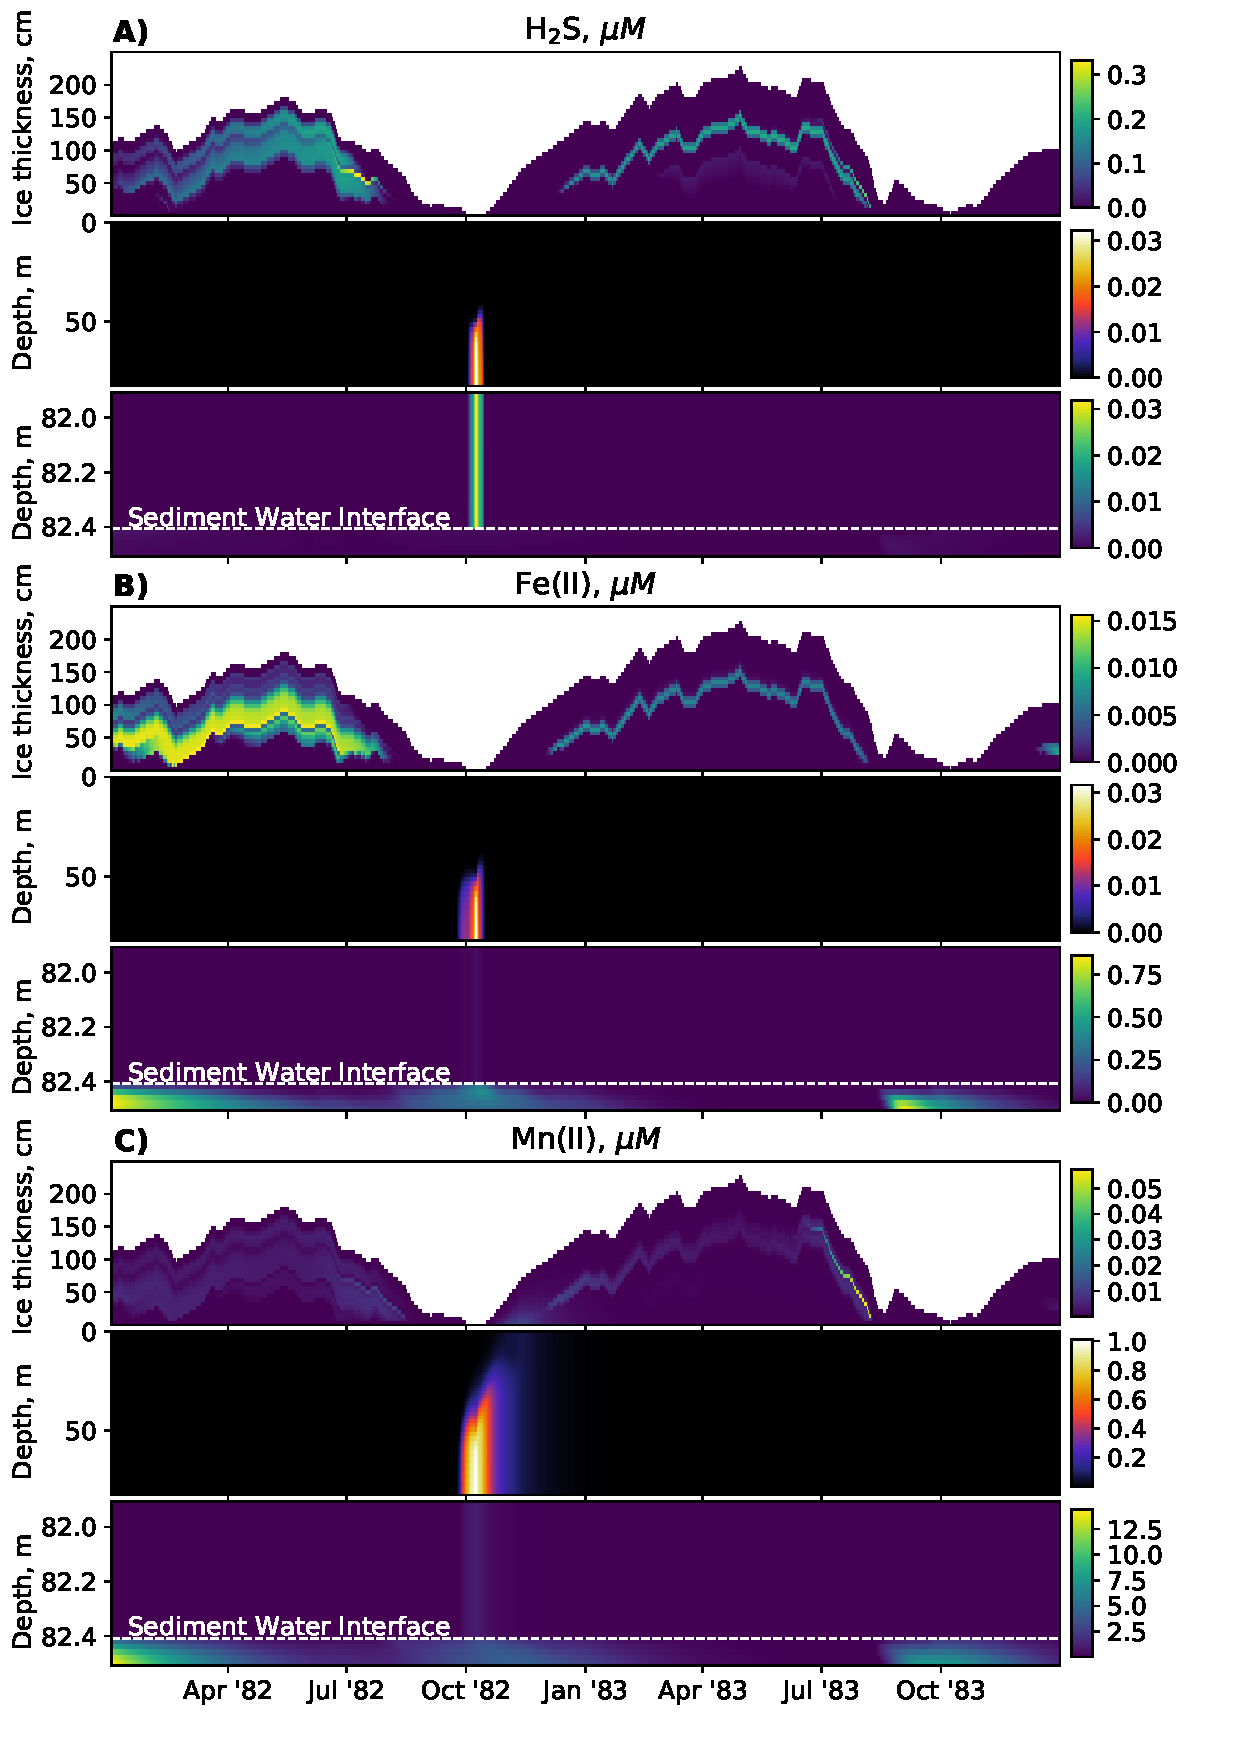
\includegraphics[width=13.6cm]{fig05_3}
\caption{Variability of \textrm{BROM} parameters}
\label{fig:brom3}
\end{figure}

In Figs.~\ref{fig:brom2} - \ref{fig:brom3} it is demonstrated that a long ice melting season leads to a strong stratification in the water column that prevents oxygen supply from the surface layer downwards.
\textrm{OM} produced during the phytoplankton bloom leads to oxygen consumption in the subsurface layers, thereby triggering the process of denitrification and the consumption of nitrate and nitrite for \textrm{OM} decomposition.
Variability of nitrogen species illustrates this as a temporal decrease of concentrations of nitrate and an increase of ammonia in the water column (Fig.~\ref{fig:brom2}).
Before and after this nitrate minimum nitrate maxima are formed.
For this oxygen depleted period the model predicts also an increase in content of dissolved \chem{Mn^{2+}} and dissolved \chem{Fe^{2+}} (Fig.~\ref{fig:brom3}b,c), connected with the reduction of oxidized forms of these metals.
Finally, trace concentrations of hydrogen sulfide appear in the bottom water (Fig.~\ref{fig:brom3}a) due to the process of sulphate reduction that starts when oxidized forms of nitrogen, manganese and iron are depleted.
This sequence of changes of electron acceptors corresponds to the theory~\citep{Canfield2009} and to the classical features of the structure of the water column redox interfaces, e.g. in the Black Sea or the Baltic Sea~\citep{Murray1995, Yakushev2006, Jost2007}.
Similar temporal changes are observed in places with variable redox conditions, e.g. Norwegian fjords and coastal lagoons~\citep{Haraldsson1988, Riguad2013, Pakhomova2014}.
The duration and intensity of oxygen depletion in the water column (and therefore in the sediments) are determined by the oxygen and \textrm{OM} supply in combination with the peculiarity of the ice regime (time and duration of the ice-melting period), that affect the distributions of chemical and biological parameters in the water column.

\section{Discussion}
\label{subsec:discussion}

Overall, the test simulations demonstrate potentially important interactions between ice, water, and sediment biogeochemistry, and how distinct vertical structure can emerge in the ice (Figs.~\ref{fig:ice_diatoms_nutrients} - \ref{fig:brom3}) and in the sediments (Figs.~\ref{fig:brom1} - \ref{fig:brom3}).
This suggests that \textrm{SPBM} is a potentially useful tool for marine biogeochemical modelling in the Arctic.
However, there are some important limitations of the present version that the user should consider.

First, as a 1D model, \textrm{SPBM} does not explicitly account for horizontal transports (advection/diffusion) which may be significant in the water column.
Horizontal mixing fluxes can however be implemented, with depth/time-varying mixing concentrations and mixing rate coefficients.
Of course this latter is more likely to give reasonable results if the real horizontal transports are of a mixing/exchange character, rather than e.g. a persistent advective flux divergence.
An alternative that could be implemented in future versions is to allow arbitrary depth/time-varying horizontal transport contributions or advective timescales to be read from file, perhaps based on a 3D biogeochemical model simulation e.g.~\citet{Friedrichs2007}.

Second, the present ice parametrization in \textrm{SPBM} is most suitable for one-year-old sea ice since it is largely based on formulations from~\citet{Arrigo1993}.
If this is not adequate, the ice brine volume and diffusion coefficients can alternatively be taken from an ice thermodynamic model (if available).
Also, the present \textrm{SPBM} implementation of gases in ice takes into account only the dissolved part of them and does not include bubbles.
Since most of the biogeochemistry processes in ice occur in brine channels it is not crucial in the context of oxygen availability for redox reactions representation.
But the fact that this process is not included can result in overestimation of initial values for dissolved gases incorporated in an ice core (e.g.~\citet{Rysgaard2004} estimate the bubbles contribute roughly a third of the total oxygen content in ice).
This will also be addressed in further work.

A third potential weakness of \textrm{SPBM} is in the parameterization of transport in the sediments (porosity, diffusion, and burial velocities).
Equations (\ref{eq:advection}, \ref{eq:burial}) assume a fixed (time-invariant) porosity profile, a fixed deep burial velocity for solutes and particulates, and no net contribution of biogeochemical transformations to the total particulate volume fraction (see~\citet{Yakushev2017} Appendix B).
This in turn implies a fixed total particulate volume flux or “sedimentation rate” at the \textrm{SWI}.
Future versions might allow some temporal variability in this total volume flux, perhaps using input files and/or including an explicit contribution from the seasonal sinking flux of \textrm{SPBM}-modelled particulates (e.g. \textrm{PON}).
A subtlety with the latter approach is that if, as in \textrm{SPBM}, the bottom layer of the water column is considered a “fluff layer” with particles entering at sinking velocity and leaving at burial velocity, then additional assumptions are required to determine the flux of modelled particulates that enters the sediments and becomes part of the sediment matrix, rather than remaining as “fluff” on the \textrm{SWI}~\citep{Yakushev2017}.
A related issue here is the lack of explicit erosion/resuspension processes in the present \textrm{SPBM} model.
Within the sediments, the neglect of solute adsorption in the present version may also be an issue in some applications.

Fourth: the ability of \textrm{FABM} to combine state variables from different models in a modular fashion (as specified in the configuration file) should accelerate the development of well-parameterized sympagic-pelagic-benthic biogeochemical modules within \textrm{SPBM}, and will also ensure that the same module code is used in any subsequent 3D simulations as long as the 3D model is also \textrm{FABM}-coupled (e.g. \textrm{ROMS}, \textrm{FVCOM}, \textrm{GETM}, \textrm{MOM}, \textrm{NEMO}).
However, care is needed to ensure compatibility between state variables, and differences in model structure and currencies may present obstacles.
For example, in test case 1 we combined state variables from \textrm{ERSEM} and \textrm{BROM}, seeking to combine the pelagic process resolution in \textrm{ERSEM} with the \textrm{BROM} resolution of redox biogeochemistry and sedimentary nutrient recycling.
However, it was not possible to fully couple these models because they use different currencies (\textrm{BROM} uses nitrogen units, while \textrm{ERSEM} uses carbon, nitrogen, phosphorus, and silicon).
Complete coupling of \textrm{ERSEM} and \textrm{BROM} may ultimately require some recoding of \textrm{BROM} state variable modules to allow for flexible elemental stoichiometry.
Furthermore, while \textrm{FABM} allows modules to be repurposed to describe domain-specific variables (e.g. ice diatoms from the \textrm{ERSEM} primary producer module in test case 1) the user must exercise caution to ensure that parameter values are suitably adapted and that the module has sufficient flexibility to describe the domain-specific variable (if not, a new \textrm{FABM} module may need to be written).
Also, a structural approximation that may be adequate in one domain (e.g. the use of one lability class for \textrm{DON} in \textrm{BROM}) may not be adequate in another (e.g. for \textrm{DON} in ice, as in test case 2).

Finally, the \textrm{SPBM} approach of simulating all variables in all domains implies some computationally inefficiency, e.g. calculating the transport of minute quantities of phytoplankton in the sediments.
Future versions could implement domain-specific screening switches to avoid this, although in a 1D context this may not be necessary.
Also, a base assumption that “everything is everywhere, but the environment selects”~\citep{OMalley2008} can be insightful.
For example in test case 1, \textrm{SPBM} simulated some limited growth of phytoplankton groups in the ice domain, and this may be important in seeding the phytoplankton blooms in the water column following ice melt~\citep{Mundy2011}.

\conclusions  %% \conclusions[modified heading if necessary]

We aimed to develop a flexible and computationally-efficient 1D vertical transport model to allow simultaneous simulation of the marine biogeochemistry of 3 different media: ice, water, and sediments.
The resulting Sympagic-Pelagic-Benthic Model (\textrm{SPBM}) includes vertically-resolved ice and sediment domains, and allows fine resolution of the benthic boundary layer.
\textrm{SPBM} reads input file data on ice growth and water column physics (and optionally also brine volumes and ice diffusivity) and uses the Framework for Aquatic Biogeochemical Models (\textrm{FABM}) to provide a user-defined model for biogeochemical transformations and water column sinking velocities, based on published models in the \textrm{FABM} library and possible new modules written by the user.
Two test simulations demonstrated the potential utility of \textrm{SPBM} for modelling systems with strong interactions between ice, water column, and sediment biogeochemistry, as are often found in the Arctic Ocean and shelf seas.
In the first test case, the \textrm{FABM} coupling was used to combine modules from two complex biogeochemical models (\textrm{ERSEM} and \textrm{BROM}) and to adapt an existing \textrm{ERSEM} diatom parameterization to simulate a new sea ice diatom group in combination with the other four \textrm{ERSEM} phytoplankton groups.
The simulation demonstrated a strong interaction between water column and ice domains with respect to algal blooms, with the ice providing seed populations of phytoplankton and the water column providing an income of nutrients.
It also demonstrated that different groups of primary producers have different spatial and temporal variabilities both in the ice and water domains due to different requirements and limitations.
A second test case demonstrated strong interactions between ice, water, and sediment domains, with spatial variability of nutrients in sea water during sea ice congelation season determining the processes occurring in the ice core in the following winter, and the melting season features determining the redox reactions occurring in the sediments.
Although there are some notable limitations of the present \textrm{SPBM} version, the results herein suggest that \textrm{SPBM} can already provide a useful tool for tuning existing biogeochemical models, accelerating the development of new biogeochemical models for regions with strong interactions between ice, water column, and sediments, and for investigating the potential importance of such interactions in determining the response of Arctic ecosystems to local and global anthropogenic drivers.

%% The following commands are for the statements about the availability of data sets and/or software code corresponding to the manuscript.
%% It is strongly recommended to make use of these sections in case data sets and/or software code have been part of your research the article is based on.

\codeavailability{It is licensed under GNU General Public License (GPL) version 2 and freely available at \url{https://github.com/BottomRedoxModel/SPBM}, (git tag v0.2)} %% use this section when having only software code available

%%\dataavailability{TEXT} %% use this section when having only data sets available


%%\codedataavailability{TEXT} %% use this section when having datasets and software code available

\appendix
\section{}    %% Appendix A
\label{app:A}

\emph{Porosity} $\varphi(z)$ at depth \unit{z} in the ice column is considered as relative volume of brine channels in ice~\citep{Arrigo1993}:
\begin{equation}
    \varphi(z) =
    \frac{\rho_{i}(z) S_{i}(z)}{\rho_{b}(z) S_{b}(z)}
\end{equation}

\emph{Brine salinity}, $S_{b}(z)$ [\unit{ppt}]~\citep{Arrigo1993} and corresponding sea ice temperature (degrees Celsius), $T_{i}(z)$:
\begin{align}
    S_{b}(z) &= \alpha_{0} + \alpha_{1} T_{i}(z)
             + \alpha_{2} T_{i}(z)^{2}
             + \alpha_{3} T_{i}(z)^{3} \\
    T_{i}(z) &= AirTemperature + \frac
               {(WaterTemperature - AirTemperature)}
               {IceThickness} z
\end{align}

where $\alpha_{0}$, $\alpha_{1}$, $\alpha_{2}$ and $\alpha_{3}$ are different for 3 ranges of temperatures:

\begin{tabular}{crrrr}
    $T_{i}$ & $\alpha_{0}$ & $\alpha_{1}$ & $\alpha_{2}$ & $\alpha_{3}$ \\
    -1.85 $ > T_{i} \ge $ -22.9 & -3.9921 & -22.700 & -1.0015   & -0.019956 \\
    -22.9 $ > T_{i} \ge $ -44   & 206.24  & -1.8907 & -0.060868 & -0.0010247 \\
    -44 $ > T_{i} \ge $ -54     & -4442.1 & -277.86 & -5.501    & -0.03669
\end{tabular}
\newline

\emph{Sea ice salinity}, $S_{i}(z)$ [\unit{ppt}]~\citep{Gerland1999, Duarte2015}:
\begin{equation}
    S_{i}(z) = 19.539 \cdot Z_{p}^{2}
             - 19.93  \cdot Z_{p}
             + 8.913
\end{equation}

where $Z_{p}$ is the ratio between the distance from the ice surface and ice thickness.

\emph{Brine density}, $\rho_{b}(z)$ [\unit{g\,m^{-3}}]~\citep{Cox1975}:
\begin{equation}
    \rho_{b}(z) = (1 + c S_{b}(z)) \cdot 10^{6}
\end{equation}

where $c = 8 \cdot 10^{-4}$ \unit{g\,m^{-3}\,ppt^{-1}}

\emph{Sea ice density}, $\rho_{i}(z)$ [\unit{g\,m^{-3}}]~\citep{Arrigo1993}:
\begin{equation}
    \rho_{i}(z) = \frac
    {\rho_{0} \rho_{b}(z) S_{b}(z)}
    {\rho_{b}(z) S_{b}(z) - S_{i}(z)
    (\rho_{b}(z) - \rho_{0})}
\end{equation}

where $\rho_{0} = 912 \cdot 10^{3}$ \unit{g\,m^{-3}} is the density of pure ice.

\section{}    %% Appendix B
\label{app:B}

The molecular diffusivity $D_{m}$ [\unit{m^{2}\,s^{-1}}] mixes concentrations of the solutes in units [\unit{mmol m^{-3}\,solutes}].
While the bioturbation diffusivity $D_{b}$ [\unit{m^{2}\,s^{-1}}] mixes concentration of the both solutes and solids in units [\unit{mmol\,m^{-3}\,total\,volume}].
So there is a flux for solutes on the \textrm{SWI}:
\begin{align}
    F_{swi} &= - \varphi_{swi} D_{m} \frac{\frac{C_{a}}{\varphi_{a}} - \frac{C_{b}}{\varphi_{b}}} {\Delta z}
    - D_{b} \frac{C_{a} - C_{b}}{\Delta z} = \\
    &= \frac{C_{a}(- \frac{\varphi_{swi}}{\varphi_{a}} D_{m} - D_{b})}{\Delta z}
    + \frac{C_{b}(  \frac{\varphi_{swi}}{\varphi_{b}} D_{m} + D_{b})}{\Delta z}
    \label{eq:b1}
\end{align}

In the 1D model the flux is calculated in the form where the porosity factor $P_{f}(z_{a,b})$ should be determined:
\begin{align}
    F_{swi} &= - \varphi_{swi}(D_{m} + D_{b})
    \frac{P_{f}(z_{a}) C_{a} - P_{f}(z_{b}) C_{b}}{\Delta z} = \\
    &= - \frac{\varphi_{swi}(D_{m} + D_{b})P_{f}(z_{a}) C_{a}}{\Delta z}
    + \frac{\varphi_{swi}(D_{m} + D_{b})P_{f}(z_{b}) C_{b}}{\Delta z}
    \label{eq:b2}
\end{align}

Comparing Eq.~(\ref{eq:b1}) and Eq.~(\ref{eq:b2}):
\begin{equation}
    P_{f}(z_{a,b}) =
    \frac{\frac{\varphi_{swi}}{\varphi_{a,b}} D_{m} + D_{b}}
    {\varphi_{swi} (D_{m} + D_{b})}
\end{equation}

And for solids since $D_{m} = 0$ and $1 - \varphi_{swi}$ instead of $\varphi_{swi}$:
\begin{equation}
    P_{f}(z_{a,b}) = \frac{1}{1 - \varphi_{swi}}
\end{equation}

where $C$ is the concentration of the variable, [\unit{mmol\,m^{-3}\,total\,volume}];
$\varphi$ is porosity, dimensionless.
Subscripts $a$, $b$ and $swi$ determinate a location of the corresponding variables: $a$ means the layer above, $b$ - the layer below, $swi$ - on the \textrm{SWI}.

\section{}    %% Appendix C
\label{app:C}

\begin{table}[H]
\centering
\caption{Common parameters}
\label{table:Common_parameters}
\begin{tabular}{lllll}
\tophline
    Parameter & Description & Value & Unit & Reference \\
\middlehline
    $t$ & Time step & 300 & \unit{s} & \\
    $D_{0}$ & Infinite-dilution molecular diffusivity & $10^{-9}$ & \unit{m^{2}\,s^{-1}} & \citep{Boudreau1997} \\
    $V_{ws}$ & Wind speed & $5$ & \unit{m\,s^{-1}} & \\
    $\chem{CO_{2}}$ (g) & Concentration of \chem{CO_{2}} in air & $380$ & \unit{ppm} & \\
\bottomhline
\end{tabular}
\belowtable{} % Table Footnotes
\end{table}

\begin{table}[H]
\centering
\caption{Ice parameters}
\label{table:Ice_parameters}
\begin{tabular}{lllll}
\tophline
    Parameter & Description & Value & Unit & Reference \\
\middlehline
    $D_{m}(s)$ & Diffusivity on sea-water interface & $10^{-5}$ & \unit{m^{2}\,s^{-1}} & \citep{Jin2008} \\
    $u_{d}$ & Diatoms vertical movement velocity & 3 & \unit{cm\,d^{-1}} \\
    $F_{vb}$ & Flux rate from the brine channels & $10^{-8}$ & \unit{m\,s^{-1}} & \citep{Arrigo1993} \\
    $z_{s}$ & Thickness of the ice layer & 0.06 & \unit{m} & \\
    $\varphi_{min}$ & Minimum porosity to enable brine convection & 0.072 (0.12) & dimensionless & \citep{Arrigo1993} \\
\bottomhline
\end{tabular}
\belowtable{} % Table Footnotes
\end{table}

\begin{table}[H]
\centering
\caption{Sediments parameters}
\label{table:Sediments_parameters}
\begin{tabular}{lllll}
\tophline
    Parameter & Description & Value & Unit & Reference \\
\middlehline
    $\varphi(z_{\infty})$ & Porosity at the infinite sediments depth & 0.8 & dimensionless & \citep{Soetaert1996} \\
    $\varphi(z_{0})$ & Porosity at the sediments-water interface & 0.95 & dimensionless & \citep{Soetaert1996} \\
    $k_{\varphi}$ & Coefficient for exponential porosity change & 0.04 & \unit{m} & \citep{Soetaert1996} \\
    $\mu_{d}$ & Relative dynamic viscosity & 0.94 & dimensionless & \citep{Boudreau1997} \\
    $K_{\chem{O_{2}}}$ & Oxygen half-saturation constant & 5 & \unit{mmol\,m^{-3}} & \citep{Yakushev2017} \\
    $z_{cb}$ & Constant bioturbation activity layer width & 0.02 & \unit{m} & \citep{Boudreau1997} \\
    $D_{bm}$ & Maximum bioturbation diffusivity & $10^{-11}$ & \unit{m^{2}\,s^{-1}} & \citep{Boudreau1997} \\
    $F_{d}$ & Bioturbation decay scale & 0.01 & \unit{m} & \citep{Boudreau1997} \\
    $u_{b}$ & Deep burial velocity & $10^{-10}$ & \unit{m\,s^{-1}} & \citep{Boudreau1997} \\
\bottomhline
\end{tabular}
\belowtable{} % Table Footnotes
\end{table}

\begin{table}[H]
\centering
\caption{Irradiance parameters}
\label{table:Irradiance_parameters}
\begin{tabular}{lllll}
\tophline
    Parameter & Description & Value & Unit & Reference \\
\middlehline
    $k_{f}$ & Factor converting irradiance to \textrm{PAR} & $0.5$ & \unit{mol\,photons\,day^{-1}\,W^{-1}} & \citep{Mobley2012} \\
    $k_{scatter}$ & Fraction of transmitted radiation & $0.97$ & dimensionless & \citep{Light2008} \\
    $A_{ice}$ & Ice albedo & $0.744$ & dimensionless & \citep{Light2008} \\
    $A_{snow}$ & Snow albedo & $0.9$ & dimensionless & \citep{Perovich2007} \\
    $k_{snow}$ & Snow light extinction coefficient & $4.3$ & \unit{m^{-1}} & \citep{Perovich2007} \\
    $k_{ice}$ & Ice light extinction coefficient & $0.93$ & \unit{m^{-1}} & \citep{Light2008} \\
\bottomhline
\end{tabular}
\belowtable{} % Table Footnotes
\end{table}

\begin{table}[H]
\centering
\caption{Forcing properties were chosen according to the values provided by \citet{Stepanova2017}}
\label{table:properties}
\begin{tabular}{llll}
\tophline
    State variable & Position & Type & Value \\
\middlehline
    $\sum{\chem{CO_{2}}}$ & water surface layer & constant & 1930 \unit{mmol\,m^{-3}\,total\,volume} \\
    \chem{Alkalinity} & water surface layer & constant & 2000 \unit{mmol\,m^{-3}\,total\,volume} \\
    $\chem{PO_{4}}$ & water surface layer & sinusoidal & $M = 0.4$,  $Phase = 130$ \\
    $\chem{NO_{3}}$ & water surface layer & sinusoidal & $M = 3$,  $Phase = 130$ \\
    $\chem{Si}$ & water surface layer & sinusoidal     & $M = 10$,  $Phase = 130$ \\
    $\chem{O_{2}}$ & water surface layer & sinusoidal  & $M = 330$,  $Phase = 130$ \\
    $DON$ & water surface layer & sinusoidal  & $M = 12.5$,  $Phase = 130$ \\
    $\sum{\chem{CO_{2}}}$ & water bottom layer & constant & 2280 \unit{mmol\,m^{-3}\,total\,volume} \\
    \chem{Alkalinity} & water bottom layer & constant & 2350 \unit{mmol\,m^{-3}\,total\,volume} \\
%    \chem{NH_{4}} & upper sediments layer & constant & 5 \unit{mmol\,m^{-3}\,total\,volume} \\
\bottomhline
\end{tabular}
\belowtable{} % Table Footnotes
\end{table}

\section{}    %% Appendix D
\label{app:D}

\begin{table}[H]
\centering
\caption{\textrm{ERSEM} photosynthesis parameters}
\label{table:ersem_parameters}
\begin{tabular}{lll}
\tophline
    Parameter & Diatom & Ice diatom \\
\middlehline
    $g$ & 1.375 & 1.210 \\
    $\alpha$ & 4 & 5.98 \\
    $\beta$ & 0.07 & 0.2 \\
\bottomhline
\end{tabular}
\belowtable{} % Table Footnotes
\end{table}

In \textrm{ERSEM} there are 4 adjustable parameters that influence gross production without affecting nutrient or temperature limitation: maximum specific productivity at reference temperature ($g$), initial slope of PI-curve ($\alpha$), photoinhibition parameter ($\beta$), and maximum effective chlorophyll to carbon photosynthesis ratio ($\phi$).
Tuning these parameters one can get different photosynthesis-irradiance curves which would represent different irradiance requirements~\citep[e.g.,][Figure 13, p.~1333]{ersem2016}.
We wanted our new primary producer functional group to be more tolerant to lower \textrm{PAR} conditions, but we did not want to change significantly its behaviour.
So we adjusted only $g$, $\alpha$, and $\beta$ in the way that increased the initial slope of the photosynthesis-irradiance curve but preserved the area under this curve from 0 to 20 $W m^{-2}$.
The parameters for the original \textrm{ERSEM} diatom and the derived parameters for the new ice diatom are presented in Table~\ref{table:ersem_parameters}.

\section{}    %% Appendix E
\label{app:E}

\citet{Rysgaard2004} reported quite large ammonium values in the ice column during a melting season.
In test case 1 we used an assumption that during spring melting all brine channels are connected ($\varphi_{min} = 0.072$ according to~\citet{Arrigo1993}), but ~\citet{Rysgaard2004} observed in the ice core simultaneous presence of \chem{O_{2}} and \chem{NH_{4}^{+}} in large concentrations, that can hardly happen in one brine volume.
To overcome this issue we changed an enabling brine convection minimum porosity parameter $\varphi_{min}$ to the larger value (0.12).
This prevented a connection in the middle part of the ice core between brine channels during the start of the melting season, thus making the modelled profile more similar to the observed values from~\citet{Rysgaard2004}.

%\subsection{}     %% Appendix A1, A2, etc.


\noappendix       %% use this to mark the end of the appendix section

%% Regarding figures and tables in appendices, the following two options are possible depending on your general handling of figures and tables in the manuscript environment:

%% Option 1: If you sorted all figures and tables into the sections of the text, please also sort the appendix figures and appendix tables into the respective appendix sections.
%% They will be correctly named automatically.

%% Option 2: If you put all figures after the reference list, please insert appendix tables and figures after the normal tables and figures.
%% To rename them correctly to A1, A2, etc., please add the following commands in front of them:

%%\appendixfigures  %% needs to be added in front of appendix figures

%%\appendixtables   %% needs to be added in front of appendix tables

%% Please add \clearpage between each table and/or figure. Further guidelines on figures and tables can be found below.



%%\authorcontribution{TEXT} %% optional section

\competinginterests{The authors declare that they have no conflict of interest.} %% this section is mandatory even if you declare that no competing interests are present

%%\disclaimer{TEXT} %% optional section

\begin{acknowledgements}
The contributions of Ph.Wallhead, E.Protsenko, and E.Yakushev were supported by the Norwegian Research Council SKATTEfunn project 272749 "Aquatic Modeling Tools", by the FRAM High North Research Centre for Climate and the Environment under projects ECOAN and OA-DREAM, and the PERMAFLUX project funded by Arctic 2030 - "The Norwegian Ministry of Foreign Affairs grant scheme in the High North". E.Protsenko and E.Yakushev also acknowledge support from grant RNF 14-50-00095.
\end{acknowledgements}




%% REFERENCES

%% The reference list is compiled as follows:

%%\begin{thebibliography}{}
%%
%%\bibitem[AUTHOR(YEAR)]{LABEL}
%%REFERENCE 1
%%
%%\bibitem[AUTHOR(YEAR)]{LABEL}
%%REFERENCE 2
%%
%%\end{thebibliography}

%% Since the Copernicus LaTeX package includes the BibTeX style file copernicus.bst,
%% authors experienced with BibTeX only have to include the following two lines:
%%
\bibliographystyle{copernicus}
\bibliography{bibtexdatabase}
%%
%% URLs and DOIs can be entered in your BibTeX file as:
%%
%% URL = {http://www.xyz.org/~jones/idx_g.htm}
%% DOI = {10.5194/xyz}


%% LITERATURE CITATIONS
%%
%% command                        & example result
%% \citet{jones90}|               & Jones et al. (1990)
%% \citep{jones90}|               & (Jones et al., 1990)
%% \citep{jones90,jones93}|       & (Jones et al., 1990, 1993)
%% \citep[p.~32]{jones90}|        & (Jones et al., 1990, p.~32)
%% \citep[e.g.,][]{jones90}|      & (e.g., Jones et al., 1990)
%% \citep[e.g.,][p.~32]{jones90}| & (e.g., Jones et al., 1990, p.~32)
%% \citeauthor{jones90}|          & Jones et al.
%% \citeyear{jones90}|            & 1990



%% FIGURES

%% When figures and tables are placed at the end of the MS (article in one-column style), please add \clearpage
%% between bibliography and first table and/or figure as well as between each table and/or figure.


%% ONE-COLUMN FIGURES

%%f
%\begin{figure}[t]
%\includegraphics[width=8.3cm]{FILE NAME}
%\caption{TEXT}
%\end{figure}
%
%%% TWO-COLUMN FIGURES
%
%%f
%\begin{figure*}[t]
%\includegraphics[width=12cm]{FILE NAME}
%\caption{TEXT}
%\end{figure*}
%
%
%%% TABLES
%%%
%%% The different columns must be seperated with a & command and should
%%% end with \\ to identify the column brake.
%
%%% ONE-COLUMN TABLE
%
%%t
%\begin{table}[t]
%\caption{TEXT}
%\begin{tabular}{column = lcr}
%\tophline
%
%\middlehline
%
%\bottomhline
%\end{tabular}
%\belowtable{} % Table Footnotes
%\end{table}
%
%%% TWO-COLUMN TABLE
%
%%t
%\begin{table*}[t]
%\caption{TEXT}
%\begin{tabular}{column = lcr}
%\tophline
%
%\middlehline
%
%\bottomhline
%\end{tabular}
%\belowtable{} % Table Footnotes
%\end{table*}
%
%
%%% MATHEMATICAL EXPRESSIONS
%
%%% All papers typeset by Copernicus Publications follow the math typesetting regulations
%%% given by the IUPAC Green Book (IUPAC: Quantities, Units and Symbols in Physical Chemistry,
%%% 2nd Edn., Blackwell Science, available at: http://old.iupac.org/publications/books/gbook/green_book_2ed.pdf, 1993).
%%%
%%% Physical quantities/variables are typeset in italic font (t for time, T for Temperature)
%%% Indices which are not defined are typeset in italic font (x, y, z, a, b, c)
%%% Items/objects which are defined are typeset in roman font (Car A, Car B)
%%% Descriptions/specifications which are defined by itself are typeset in roman font (abs, rel, ref, tot, net, ice)
%%% Abbreviations from 2 letters are typeset in roman font (RH, LAI)
%%% Vectors are identified in bold italic font using \vec{x}
%%% Matrices are identified in bold roman font
%%% Multiplication signs are typeset using the LaTeX commands \times (for vector products, grids, and exponential notations) or \cdot
%%% The character * should not be applied as mutliplication sign
%
%
%%% EQUATIONS
%
%%% Single-row equation
%
%\begin{equation}
%
%\end{equation}
%
%%% Multiline equation
%
%\begin{align}
%& 3 + 5 = 8\\
%& 3 + 5 = 8\\
%& 3 + 5 = 8
%\end{align}
%
%
%%% MATRICES
%
%\begin{matrix}
%x & y & z\\
%x & y & z\\
%x & y & z\\
%\end{matrix}
%
%
%%% ALGORITHM
%
%\begin{algorithm}
%\caption{}
%\label{a1}
%\begin{algorithmic}
%
%\end{algorithmic}
%\end{algorithm}
%
%
%%% CHEMICAL FORMULAS AND REACTIONS
%
%%% For formulas embedded in the text, please use \chem{}
%
%%% The reaction environment creates labels including the letter R, i.e. (R1), (R2), etc.
%
%\begin{reaction}
%%% \rightarrow should be used for normal (one-way) chemical reactions
%%% \rightleftharpoons should be used for equilibria
%%% \leftrightarrow should be used for resonance structures
%\end{reaction}
%
%
%%% PHYSICAL UNITS
%%%
%%% Please use \unit{} and apply the exponential notation


\end{document}
